%! TEX root = C:\Users\osval\OneDrive - Instituto Politecnico Nacional\Codigos\Programacion\DLP\Practica_1\main.tex

En esta práctica se busca que el estudiante se familiarice con el uso de lenguajes de descripción de hardware (HDL), principalmente VHDL y Verilog, para implementar y simular circuitos digitales dentro de una tarjeta de desarrollo FPGA. 

Los circuitos a desarrollar incluyen tanto sistemas combinacionales como secuenciales: funciones lógicas básicas a partir de una tabla de verdad, un registro de 8 bits basado en flip-flops tipo D, un contador binario ascendente/descendente de 4 bits con salida a un display de 7 segmentos, así como generadores de sonido (sirenas). 

Finalmente, se integrarán los módulos en un \textit{Top Level Design} (TLD), el cual permite concentrar todas las funciones en un único diseño jerárquico. De esta forma, el alumno recorre todo el flujo de diseño digital: codificación, simulación, síntesis, implementación y prueba en hardware real, aplicando conocimientos teóricos a aplicaciones prácticas.

\subsection*{Registro 8 bits}

Un registro de 8 bits es un circuito electrónico para el almacenamiento y proceso de datos de 8 bits.

Para el desarrollo del registro de 8 bits se va a tomar como base el uso de un flip flop tipo D (Figura: \ref{fig:FF-D}) el cual funciona para guardar un bit de la entrada D en el momento en el que exista un flanco de subida en la entrada del CLK, y este se va a mostrar en la salida Q, y en la salida Q' se va a mostrar el estado en el que se encontraba la entrada D antes del cambio del flanco de subida en el CLK. 

\begin{figure}[H]
    \centering
        \resizebox{0.2\linewidth}{!}{
    \begin{tikzpicture}
	% Paths, nodes and wires:
	\node[flipflop D] at (4.453, 5.827){};
	\draw[-latex] (2.667, 6.667) -- (3.333, 6.667);
	\draw[-latex] (2.667, 5) -- (3.333, 5);
	\draw[-latex] (5.573, 6.667) -- (6.24, 6.667);
	\draw[-latex] (5.573, 4.987) -- (6.24, 4.987);
    \end{tikzpicture}
}
    \caption{Flip-Flop D}
    \label{fig:FF-D}

\end{figure}

\subsection*{Contador 4 bits Display de 7 segmentos}

Para la visualización del contador de 4 bits vamos a tener apoyo de un display de 7 segmentos de 4 dígitos (Figura: \ref{fig:display}) que viene incluido en la tarjeta de desarrollo cyclone 4.

El display de 7 segmentos es un elemento que nos permite visualizar números y letras dependiendo una combinación adecuada en los pines de entrada (a-f) y dado que esta construido por didos leds necesita una corriente máxima la cual es limitada por una resistencia que ya viene incluida de igual forma en la tarjeta de desarrollo, y al ser un display de 4 dígitos tiene 4 pines extras para definir que dígito es que que vamos a mostrar.

\begin{figure}[H]
    \centering
    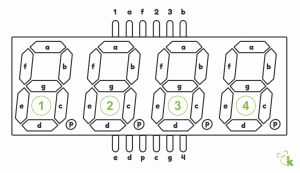
\includegraphics[width=0.5\linewidth]{imagenes/7_segmenos.png}
    \caption{Display de 7 segmentos 4 dígitos cátodo común}
    \label{fig:display}
\end{figure}


\subsection*{Modulo de Voz.}

El módulo ISD1820 es un grabador y reproductor de voz basado en el chip ISD1820. Su funcionamiento se centra en capturar, almacenar y reproducir mensajes de audio.

Utiliza un micrófono integrado para capturar el sonido. Al presionar el botón REC, el chip almacena la señal de audio de forma analógica en una memoria no volátil, donde la duración de la grabación es de aproximadamente 10 segundos.

Existen 2 modos para su reproducción.
PLAYE (Playback, Edge-activated): Al presionarlo una vez, reproduce el mensaje completo grabado.

PLAYL (Playback, Level-activated): Mientras se mantiene presionado, reproduce el mensaje de forma continua. Al soltarlo, la reproducción se detiene.

Control: Puede operarse manualmente con sus botones o de forma automática de forma externa enviando señlaes a sus pines de control (REC, PLAYE, PLAYL).

El chip incluye un amplificador de audio interno para manejar altavoces pequeños de aproximadamente 8 ohms y 0.5 Watts.

\begin{figure}[H]
    \centering
    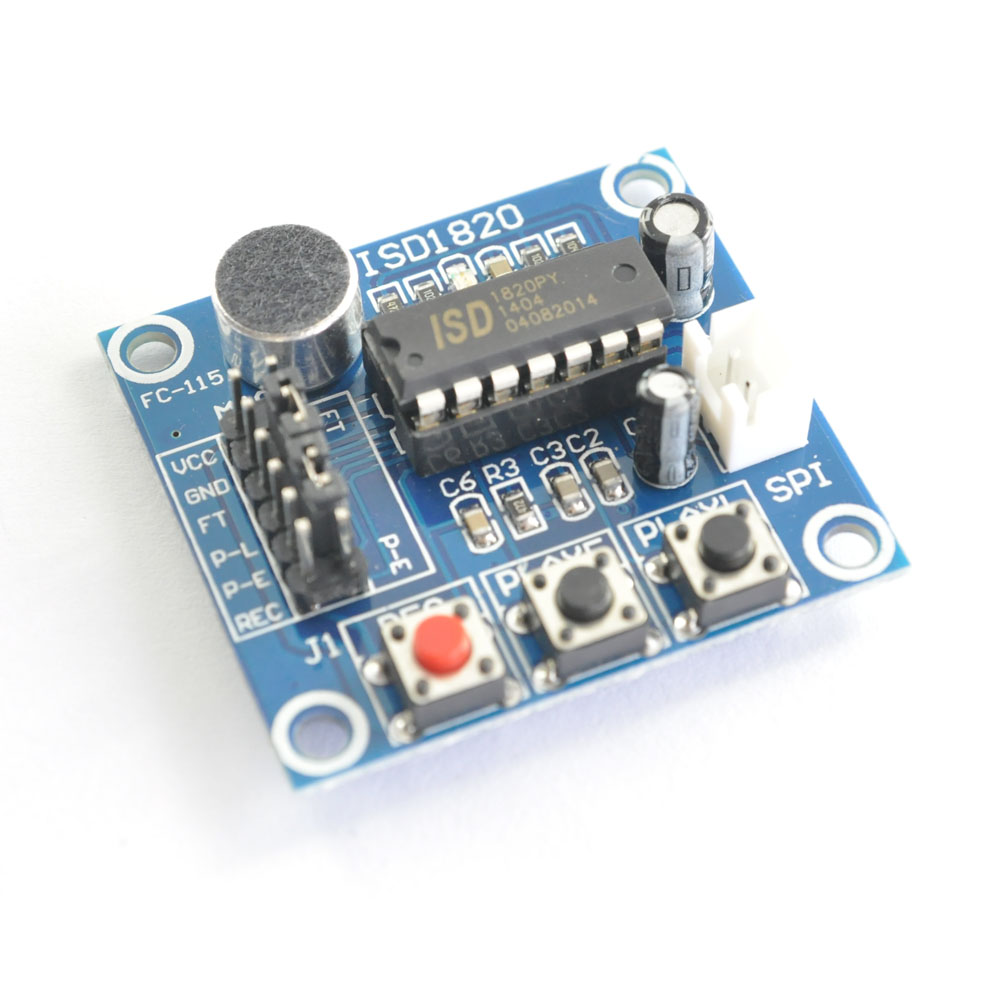
\includegraphics[width=0.5\linewidth]{imagenes/Modulo de voz.png}
    \caption{Modulo ISD1820}
    \label{fig:Voz}
\end{figure}

\subsection*{Comunicación RS232}

RS232 es una forma de comunicación en serie, lo que significa que la información se envía entre dispositivos un bit a la vez. Es una forma de comunicación asincrónica, lo que significa que los dispositivos de envío y recepción pueden operar en diferentes momentos.

El estándar RS232 define los detalles de cómo se envían y reciben los datos entre dispositivos. Las principales características del estándar RS232 son las siguientes:

Niveles de voltaje: La comunicación RS232 usa señales de voltaje para representar datos binarios. Un voltaje entre -3 V y -15 V representa un "1" binario (también conocido como "Marca"), mientras que un voltaje entre +3 V y +15 V representa un "0" binario (también conocido como "Espacio").
Transmisión de datos: RS232 admite comunicación dúplex completo, lo que significa que los datos se pueden enviar y recibir en ambas direcciones al mismo tiempo.
enmarcado: Cada paquete de datos enviado a través de RS232 contiene un bit de inicio, de 5 a 9 bits de datos, un bit de paridad opcional para la detección de errores y uno o dos bits de parada. Esta estructura se denomina "marco".
Tasa de baudios: La tasa de baudios es el número de cambios de señal por segundo que se envían o reciben a través de la línea. En RS232, la velocidad en baudios generalmente se especifica en bits por segundo (bps).
Líneas de control: RS232 utiliza varias líneas de control para gestionar el flujo de datos entre el transmisor y el receptor. Estos incluyen líneas como "Terminal de datos listo" (DTR), "Conjunto de datos listo" (DSR), "Solicitud de envío" (RTS) y "Listo para enviar" (CTS).
Comprobación de paridad: Este es un método para detectar errores en los datos transmitidos. La verificación de paridad agrega un bit adicional (el bit de paridad) a cada palabra de datos (generalmente un byte), que se establece para garantizar que el número total de 1 bits en la palabra (incluido el bit de paridad) sea siempre par o impar, según dependiendo de si se usa paridad par o impar.

